\documentclass{article}
\usepackage{pgfplots}
\pgfplotsset{compat=1.18}

\begin{document}

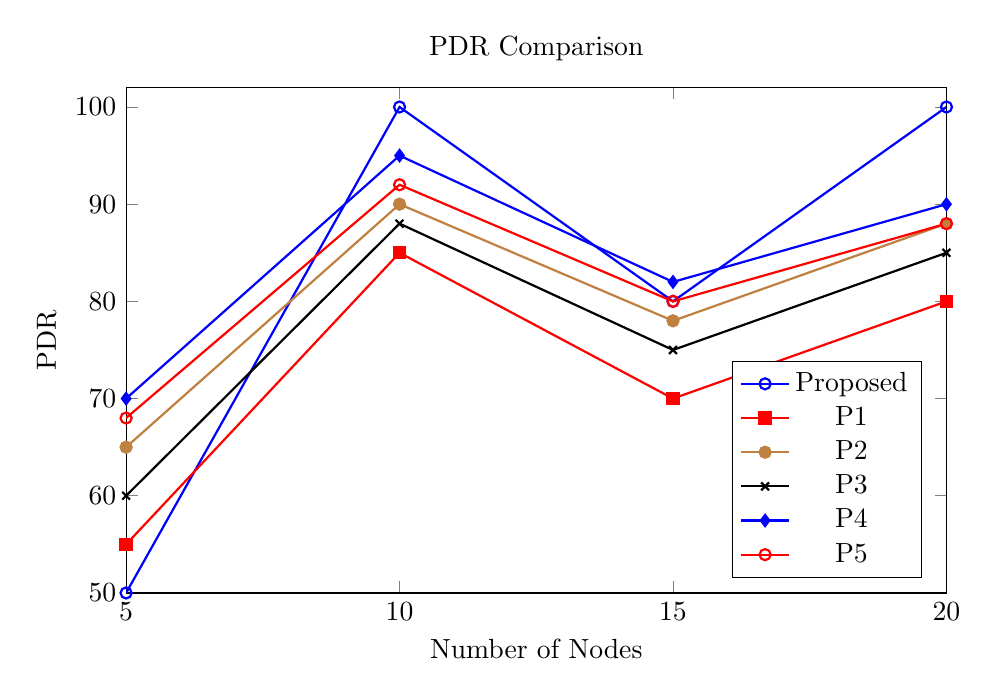
\begin{tikzpicture}
\begin{axis}[
width=12cm,
height=8cm,
title={PDR Comparison},
xlabel={Number of Nodes},
ylabel={PDR},
xmin=5, xmax=20,
ymin=50, ymax=102,
xtick={5,10,15,20},
ytick={50,60,70,80,90,100},
legend pos=south east
]

% Proposed
\addplot[solid, blue, mark=o, thick] 
coordinates {(5,50) (10,100) (15,80) (20,100)};

% P1
\addplot[solid, red, mark=square*, thick] 
coordinates {(5,55) (10,85) (15,70) (20,80)};

% P2
\addplot[solid, brown, mark=*, thick] 
coordinates {(5,65) (10,90) (15,78) (20,88)};

% P3
\addplot[solid, black, mark=x, thick] 
coordinates {(5,60) (10,88) (15,75) (20,85)};

% P4
\addplot[solid, blue, mark=diamond*, thick] 
coordinates {(5,70) (10,95) (15,82) (20,90)};

% P5 (NOW SOLID — NOT DASHED)
\addplot[solid, red, mark=o, thick] 
coordinates {(5,68) (10,92) (15,80) (20,88)};

\legend{Proposed, P1, P2, P3, P4, P5}

\end{axis}
\end{tikzpicture}

\end{document}